%%%%%%%%%%%%%%%%%%%%%%%%%%%%%%%%%%%%%%
%%%%%%%%%%%%%%%%%%%%%%%%%%%%%%%%%%%%%%
% Do not edit the TeX file your work
% will be overwritten.  Edit the RnW
% file instead.
%%%%%%%%%%%%%%%%%%%%%%%%%%%%%%%%%%%%%%
%%%%%%%%%%%%%%%%%%%%%%%%%%%%%%%%%%%%%%




% TODO: define these in knitr instead.
% \global\long\def\splinedegree{3}
% \global\long\def\ntime{14}
% \global\long\def\ngenes{1000}
% \global\long\def\nclusters{18}
% \global\long\def\fullparamdim{66199}
% \global\long\def\covregularization{0.1}
%
% \global\long\def\regmat{X_{df}}
% \global\long\def\mbe{\mathbb{E}}
% \global\long\def\cov{\mathrm{Cov}}
% \global\long\def\thetareg{\theta_{r}}
% \global\long\def\thetaclust{\theta_{c}}

\paragraph{Experimental Results for $\alpha$ Perturbations.}

We start with some DP prior parameter $\alpha_0$. After choosing a different
$\alpha$, we compare the posterior expected number of clusters (
\prettyref{eq:expected_num_clusters}) predicted by our linear approximation
against the expectation obtained from re-optimizing the objective. The results
are shown in \prettyref{fig:parametric_sens_e_num_clusters}.

More specifically, we evaluated the expected number of clusters for a range of
$\alpha$ between 0.5 and 6.5. Then we chose three $\alpha_0$ values, 2, 3.5, and
5, and constructed the linear approximation centered at each of these
$\alpha_0$s. The linear approximation did quite well for choices of $\alpha$
close to $\alpha_0$. Hence, by evaluating the objective at three $\alpha_0$s, we
can use the linear approximation to understand the effect of the DP prior
parameter $\alpha$ across the entire range from 0.5 - 6.5.


\begin{knitrout}
\definecolor{shadecolor}{rgb}{0.969, 0.969, 0.969}\color{fgcolor}\begin{figure}[!h]

{\centering 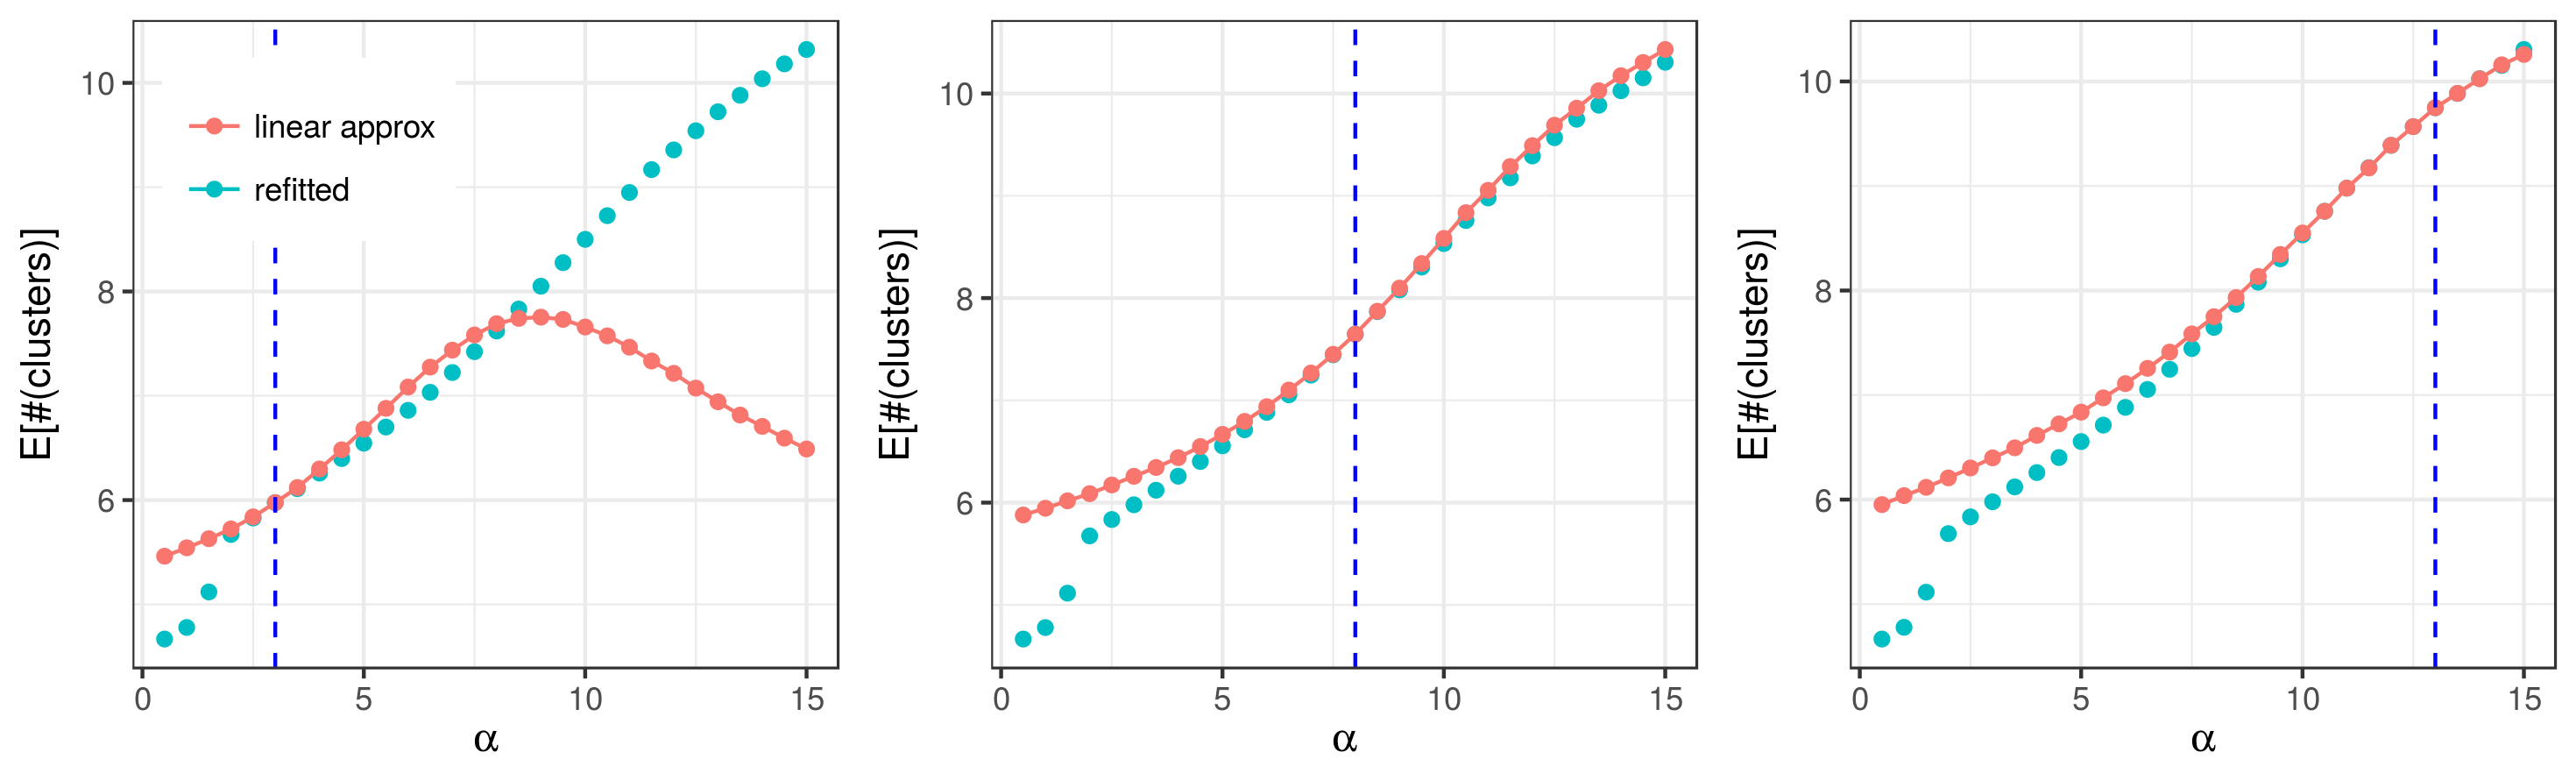
\includegraphics[width=0.98\linewidth,height=0.343\linewidth]{figure/parametric_sens_plot-1} 

}

\caption{\label{fig:parametric_sens_e_num_clusters}Comparison of the expected number of clusters computed by re-optimizing
  the variational objective for various epsilon perturbations to the BNP prior parameter
  (green),
  versus the predicted value from our linear approximation (orange), with alpha0 the
  blue horizontal line.}\label{fig:parametric_sens_plot}
\end{figure}


\end{knitrout}
